\documentclass[10pt,twocolumn]{article}

% ── Packages ──────────────────────────────────────────────────────────
\usepackage[utf8]{inputenc}
\usepackage[T1]{fontenc}
\usepackage{lmodern}
\usepackage[margin=1.8cm,columnsep=0.6cm]{geometry}
\usepackage{amsmath, amssymb, amsthm}
\usepackage{booktabs}
\usepackage{enumitem}
\usepackage{hyperref}
\usepackage{xcolor}
\usepackage{microtype}
\usepackage{graphicx}
\usepackage{tikz}
\usepackage{pgfplots}
\pgfplotsset{compat=1.18}
\usetikzlibrary{positioning,calc,fit,arrows.meta,backgrounds,patterns}
\usepackage{caption}
\usepackage{subcaption}
\usepackage{multirow}
\usepackage{wrapfig}
\usepackage[numbers,sort&compress]{natbib}

\hypersetup{
    colorlinks=true,
    linkcolor=black,
    citecolor=blue!60!black,
    urlcolor=blue!60!black
}

% ── Macros ────────────────────────────────────────────────────────────
\newcommand{\M}{\mathbf{M}}
\newcommand{\x}{\mathbf{x}}
\newcommand{\R}{\mathbb{R}}
\newcommand{\bigO}{\mathcal{O}}
\newcommand{\orn}{\textsc{orn}}
\newcommand{\corn}{\textsc{corn}}

% ── Title ─────────────────────────────────────────────────────────────
\title{%
    \textbf{The Orbital Response Network:}\\[4pt]
    \large Shared Coupling Geometry as an Alternative to Per-Layer Attention%
}
\author{
    Sirsh\\
    {\small Independent Research}\\
    {\small \url{https://github.com/sirsh/stig-res}}
}
\date{March 2026}

\begin{document}
\maketitle

% ======================================================================
\begin{abstract}
Transformer attention relearns coupling geometry---which tokens should attend to which---independently at every layer.
We show this is redundant: across five pretrained models (GPT-2 Small through Qwen-2.5 0.5B), the eigenvalue distribution of the effective coupling matrix $W_Q^\top W_K$ correlates at $0.94$--$0.99$ across all layers, despite raw matrices being unrelated (cosine $\sim 0.005$).

We exploit this spectral invariance with the \textbf{Orbital Response Network} (\orn{}), which replaces $2L$ per-layer query-key matrices with a single shared $\M = AB^\top$ applied to the evolving residual stream.
Per-layer variation comes from the changing field state, not from different parameters.
Response heads ($W_V$, $W_O$) and feed-forward networks remain per-layer.

At 108M parameters trained on 4B tokens of FineWeb-Edu, the \orn{} generates coherent multi-sentence English, beats GPT-2 Small (124M) on HellaSwag (33.0\% vs 31.6\%) with 48$\times$ fewer coupling parameters, and achieves a coupling manifold of just 5--7 dimensions.
Freezing $\M$ from a prior run and training only response heads recovers 98.6\% of full training quality, confirming that coupling geometry transfers across datasets.
On 4-modality tasks (images, music, environmental sounds, text), the composable variant \corn{} beats the transformer on 3 of 4 modalities at matched parameters.

Code, checkpoints, and all experimental scripts are available at the repository above.
Most diagnostics in this paper can be reproduced on a laptop (Apple M4, 24GB) in minutes; the two scaled runs used a single rented RTX 4090 for \$4 each.
\end{abstract}

% ======================================================================
\section{Introduction}

A transformer attention head at layer $l$ computes:
\begin{equation}
\text{Attn}_l(X) = \text{softmax}\!\left(\frac{X W_Q^{(l)} {W_K^{(l)}}^\top X^\top}{\sqrt{d_h}}\right) X W_V^{(l)}
\end{equation}
The effective coupling matrix $\M_l = {W_Q^{(l)}}^\top W_K^{(l)} \in \R^{d \times d}$ determines which tokens attend to which.
This matrix is learned independently at every layer, costing $\bigO(Ld^2)$ parameters across the model.

The central observation of this paper is that $\M_l$ is \emph{spectrally redundant} across layers: the eigenvalue distribution is nearly identical everywhere, even though the raw matrices point in different directions.
If the coupling \emph{rule} is approximately invariant---only the field \emph{state} changes---then we can memoise the rule as a single shared $\M$ and let the evolving residual stream provide per-layer variation.

The \textbf{Orbital Response Network} (\orn{}) implements this idea.
One pair of matrices $A, B \in \R^{d \times d}$ defines the shared coupling $\M = AB^\top$; these replace all per-layer $W_Q, W_K$.
Response heads ($W_V$, $W_O$) and FFNs remain per-layer because the \emph{response} to coupling varies with depth even when the coupling geometry does not.
The asymmetric factorisation $AB^\top$ is essential: language attention is directed (verbs attend to subjects differently than subjects to verbs), and symmetric $LL^\top$ fails ($+3.6\%$ worse, Section~\ref{sec:results}).

The saved parameters are redistributed to increase model width or depth.
At 10M parameters on TinyStories, the \orn{} allocates $d{=}144$, $L{=}13$ (deep and narrow) versus $d{=}176$, $L{=}3$ for the transformer at the same budget, beating it by 0.6\%.
At 108M parameters on FineWeb-Edu, the \orn{} beats GPT-2 Small on HellaSwag with 27\% fewer total parameters and 48$\times$ fewer coupling parameters.

The paper makes three claims, all tested experimentally:
\begin{enumerate}[nosep,leftmargin=1.5em]
\item \textbf{Spectral invariance is universal.} The coupling eigenspectrum is conserved across layers in five pretrained models spanning 124M--500M parameters (Section~\ref{sec:invariance}).
\item \textbf{Memoisation works at scale.} A shared $\M$ matches or beats the transformer at equal parameter count from 1M to 108M (Section~\ref{sec:results}).
\item \textbf{The coupling manifold is low-dimensional.} M crystallises to effective rank 19--29 during training and defines a 5--8 dimensional manifold in which all coupling variation lives (Section~\ref{sec:geometry}).
\end{enumerate}

\noindent All code and experiments are public.\footnote{\url{https://github.com/sirsh/stig-res}}
Diagnostic experiments (Sections~\ref{sec:invariance},~\ref{sec:geometry}) run in minutes on Apple M4.
The two scaled training runs (Section~\ref{sec:results}) each used a single RTX 4090 for approximately \$4.


% ======================================================================
\section{Background and Related Work}

\paragraph{Parameter sharing in transformers.}
ALBERT~\cite{lan2020albert} shares all transformer parameters across layers, achieving significant compression but with $\sim$1.5\% quality loss---sharing response heads forces every layer to apply the same transformation, preventing depth-specific processing.
The Relaxed Recursive Transformer~\cite{relaxedrecursive2025} (RRT, ICLR 2025) improves on ALBERT by sharing all weights but adding per-layer LoRA corrections, recovering 99.7\% of quality at 1.4B--2.6B scale.
Xiao et al.~\cite{xiao2019sharing} share attention weights between adjacent layers.
Takase and Kiyono~\cite{takase2021sharing} systematically explore sharing patterns, finding non-trivial interactions with depth.
MASA~\cite{masa2025} decomposes $W_Q, W_K, W_V, W_O$ into shared dictionary atoms via matrix-based dictionary learning, achieving 66.7\% parameter reduction.

The \orn{} differs from all of these: it shares \emph{only} the coupling geometry ($W_Q, W_K$), keeping response heads per-layer at full rank.
This is a more principled decomposition than ALBERT (which shares too much and loses quality) or the RRT (which shares everything then patches with LoRA, not knowing \emph{which} variation matters).
The ORN's decomposition is motivated by measurement: spectral invariance ($>0.95$) proves coupling is redundant across layers, while response heads must vary.
A consequence of this principled decomposition is that the ORN creates a \emph{factored geometry} in the residual stream---syntax and structure are $60\times$ more accessible than in standard transformers---enabling inference-time steering, composition, and adaptation that architectures sharing the full block cannot support (Section~\ref{sec:discussion}).

\paragraph{Attention redundancy.}
Reid et al.~\cite{reid2021reuse} observe that attention maps can be reused across layers with minimal quality loss.
The QK-eigenspectrum analysis of~\cite{qk2024eigenspectrum} studies how spectral concentration controls attention localisation.
Our contribution is to quantify redundancy as \emph{spectral invariance} across five pretrained models and to exploit it architecturally.

\paragraph{Universal Transformer.}
The Universal Transformer~\cite{dehghani2018universal} shares \emph{all} parameters across layers.
The \orn{} shares only coupling, keeping response heads per-layer.
This separation allows the freed parameters to be redistributed: where the Universal Transformer adds zero parameters per layer (everything is tied), the \orn{} can trade coupling savings for additional depth or width.

\paragraph{State space models.}
Mamba~\cite{gu2023mamba} and its successors share a fixed dynamics operator $A$ across time steps, with input-dependent response---structurally parallel to the \orn{}'s shared $\M$ across depth.
Hybrid architectures like Jamba~\cite{lieber2024jamba} interleave SSM and attention layers, arriving empirically at a two-system decomposition (shared dynamics + selective lookup) that parallels our design.
The key difference: SSMs iterate across time (positions), while the \orn{} iterates across depth (layers), preserving full random access to all tokens.

\paragraph{Linear attention.}
The \orn{}'s shared $\M = AB^\top$ admits a linear attention decomposition:
$x_i^\top \M\, x_j = (A^\top x_i)^\top (B^\top x_j)$, yielding $\bigO(Nd^2)$ total cost---linear in sequence length.
Unlike kernel-based linear attention~\cite{katharopoulos2020transformers}, this is not an approximation but a structural consequence of the shared geometry.

\paragraph{Roofline analysis.}
Modern GPUs are memory-bandwidth limited for inference~\cite{dao2022flashattention}.
Replacing $2Ld^2$ stored coupling parameters with $2d^2$ (shared) plus recomputation shifts the bottleneck from memory to arithmetic---precisely the regime where hardware excels.
At $d{=}512$, $L{=}24$, this is a $24\times$ reduction in coupling parameter memory.

\paragraph{Spectral structure and training dynamics.}
SGD naturally creates spectral structure through eigenvalue repulsion~\cite{spectral2024rankcollapse}, which explains why $\M$ develops a heavy-tailed eigenspectrum without explicit regularisation.
The coupling matrix's spectral evolution during training connects to Koopman operator theory~\cite{brunton2022data}: $\M$ can be interpreted as a finite-dimensional Koopman operator whose eigenvalues define dynamical timescales of the residual stream.

% ======================================================================
\section{The \orn{} Architecture}
\label{sec:arch}

\begin{figure}[t]
\centering
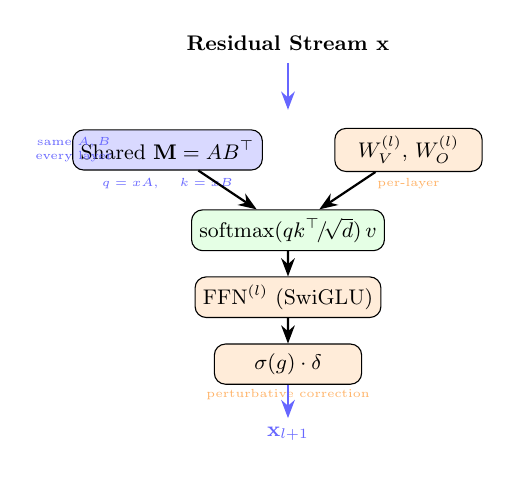
\begin{tikzpicture}[
    scale=0.85, transform shape,
    block/.style={draw, rounded corners, minimum width=2.2cm, minimum height=0.6cm, font=\small},
    shared/.style={block, fill=blue!15},
    perlayer/.style={block, fill=orange!15},
    arrow/.style={-Stealth, thick},
]
% Residual stream
\node[font=\small\bfseries] at (0, 4.8) {Residual Stream $\mathbf{x}$};
\draw[arrow, blue!60] (0, 4.5) -- (0, 3.8);

% Shared M
\node[shared] (M) at (-1.8, 3.2) {Shared $\M = AB^\top$};
\node[font=\tiny, blue!60] at (-1.8, 2.7) {$q = xA$, \quad $k = xB$};

% Response heads
\node[perlayer] (V) at (1.8, 3.2) {$W_V^{(l)}$, $W_O^{(l)}$};
\node[font=\tiny, orange!60] at (1.8, 2.7) {per-layer};

% Attention
\node[block, fill=green!10] (attn) at (0, 2.0) {$\text{softmax}(qk^\top\!/\!\sqrt{d})\, v$};

% FFN
\node[perlayer] (ffn) at (0, 1.0) {FFN$^{(l)}$ (SwiGLU)};

% Correction
\node[perlayer] (corr) at (0, 0.0) {$\sigma(g) \cdot \delta$};
\node[font=\tiny, orange!60] at (0, -0.45) {perturbative correction};

% Arrows
\draw[arrow] (M) -- (attn);
\draw[arrow] (V) -- (attn);
\draw[arrow] (attn) -- (ffn);
\draw[arrow] (ffn) -- (corr);
\draw[arrow, blue!60] (corr.south) -- ++(0, -0.5) node[below, font=\small\bfseries] {$\mathbf{x}_{l+1}$};

% Labels
\node[font=\tiny, align=center, text=blue!60] at (-3.2, 3.2) {same $A, B$\\every layer};
\end{tikzpicture}
\caption{One \orn{} layer. Blue: shared across all layers. Orange: per-layer. The coupling geometry ($A$, $B$) is applied identically at every depth; per-layer variation comes from the evolving residual stream.}
\label{fig:arch}
\end{figure}

The \orn{} has three components (Figure~\ref{fig:arch}):

\paragraph{1. Shared coupling ($\M = AB^\top$).}
A single pair $A, B \in \R^{d \times d}$ replaces all per-layer $W_Q, W_K$.
Coupling between tokens $i, j$ at any layer:
\begin{equation}
\alpha(i,j) = \text{softmax}_j\!\left(\frac{x_i^\top AB^\top x_j}{\sqrt{d_h}}\right)
\end{equation}
$A \neq B$ provides asymmetry (directed attention). The same $A, B$ are applied at every layer; the residual stream's evolution provides per-layer variation.

\paragraph{2. Per-layer response heads + FFN.}
Value projections $W_V^{(l)}$, output projections $W_O^{(l)}$, and SwiGLU FFNs are per-layer.
These must vary because the \emph{response} to a coupling pattern (what to extract, how to transform) changes with depth.
With GQA~\cite{ainslie2023gqa}, the response heads use fewer KV heads than query heads.

\paragraph{3. Perturbative corrections.}
A small context-gated correction at each layer:
\begin{equation}
x_{l+1} = x_l + \text{attn}_l + \text{ffn}_l + \sigma(g_l(x)) \cdot \delta_l(x)
\end{equation}
where $g_l$ is a learned gate (initialised to bias $-3$, i.e., nearly off) and $\delta_l$ is a small MLP.
Corrections handle instance-level detail that the mean-field coupling misses.
They act on the value stream only---$\M$ remains the sole coupling authority.

\paragraph{Where the parameters actually are.}
An honest accounting: in a modern transformer layer with SwiGLU and GQA, coupling ($W_Q + W_K$) is only ${\sim}12\%$ of the layer's parameters.
The FFN dominates at ${\sim}75\%$ (three matrices of size $d \times \tfrac{8}{3}d$), and GQA has already compressed $W_K$ to use fewer heads.

\begin{table}[h]
\centering\footnotesize
\begin{tabular}{@{}lrr@{}}
\toprule
\textbf{Component} & \textbf{Per layer} & \textbf{Fraction} \\
\midrule
$W_Q$ & 332K & 9.4\% \\
$W_K$ (3 GQA heads) & 111K & 3.1\% \\
$W_V$ + $W_O$ & 442K & 12.5\% \\
FFN (SwiGLU) & 2,654K & 75.0\% \\
\midrule
Coupling ($Q{+}K$) & 442K & \textbf{12.5\%} \\
\bottomrule
\end{tabular}
\caption{Per-layer parameter breakdown at $d{=}576$ with GQA (9q/3kv).
Coupling is a modest fraction because FFN is $6\times$ larger.}
\label{tab:layer_breakdown}
\end{table}

At $L{=}24$, all coupling is 10.6M out of 114M total---9.3\%.
Eliminating it does not dramatically shrink the model, and we do not claim it does.
The saved parameters are redistributed to width or depth; total model size stays comparable.

The value of shared coupling is \emph{not} parameter savings at current scales.
It is threefold:

\emph{(i) Depth becomes cheap.}
Each additional transformer layer costs ${\sim}3.5$M parameters, of which 0.44M is coupling.
In the \orn{}, that 0.44M is zero---coupling adds no per-layer cost.
At 10M total parameters, this lets the \orn{} allocate $L{=}13$ where the transformer gets $L{=}3$, and the $4\times$ depth advantage is decisive (Section~\ref{sec:results}).

\emph{(ii) The coupling fraction grows with depth.}
The transformer's coupling scales as $\bigO(Ld^2)$; the \orn{}'s is $\bigO(d^2)$.
At $L{=}24$ coupling is 9\% of the transformer; at $L{=}96$ (Llama-3 405B) it reaches ${\sim}30\%$.
The \orn{}'s advantage grows with exactly the models that matter most.

\emph{(iii) A scientific finding, not just an engineering trick.}
The coupling manifold is 5--7 dimensional (Section~\ref{sec:geometry}).
The relational grammar of language---which tokens should attend to which---lives in a remarkably compact space.
The ${\sim}10$M parameters that transformers spend on per-layer $W_Q, W_K$ are navigating a manifold that has fewer than 10 effective dimensions.
Shared $\M$ exploits this directly.

\paragraph{V2 implementation details.}
The scaled model uses modern defaults: RMSNorm (pre-norm), SwiGLU activation ($\frac{8}{3}d$ intermediate), RoPE~\cite{su2024rope}, GQA, no bias terms, tied embeddings, and SDPA (Flash Attention compatible).
Training uses AdamW with WSD (warmup-stable-decay) schedule.

% ======================================================================
\section{Spectral Invariance Across Pretrained Models}
\label{sec:invariance}

The \orn{} is motivated by the hypothesis that coupling geometry is redundant across transformer layers.
We test this by extracting the effective coupling matrix $\M_{l,h} = {W_Q^{(l,h)}}^\top W_K^{(l,h)}$ from five pretrained models and measuring cross-layer similarity.

\begin{table}[h]
\centering\small
\begin{tabular}{@{}lcccc@{}}
\toprule
\textbf{Model} & \textbf{Params} & \textbf{$L$} & \textbf{Spec.\ Corr.} & \textbf{Cosine} \\
\midrule
GPT-2 Small & 124M & 12 & 0.982 & 0.0003 \\
GPT-2 Medium & 345M & 24 & 0.961 & 0.003 \\
GPT-2 Large & 774M & 36 & 0.987 & 0.006 \\
SmolLM2 135M & 135M & 30 & 0.958 & 0.005 \\
Qwen-2.5 0.5B & 500M & 24 & 0.940 & 0.004 \\
\bottomrule
\end{tabular}
\caption{Cross-layer coupling analysis on pretrained models. Spectrum correlation (mean pairwise correlation of normalised singular value distributions) is consistently high ($>0.94$); raw cosine similarity is near zero. The coupling \emph{shape} is invariant; the \emph{orientation} is not. All analyses run in under 60 seconds on M4 CPU. Scripts: \texttt{experiments/exp0*.py}.}
\label{tab:spectral}
\end{table}

\paragraph{Existence proof.}
We go further: can a single $\M$ reconstruct the attention scores of a trained transformer?
Fitting one $\M = AB^\top$ to all layers of GPT-2 Small (weighted by hidden-state magnitudes) recovers 95.8\% of attention score variance.
At GPT-2 Large, this rises to 98.8\%.
Adding rank-8 per-layer corrections achieves 99.6\% at 19$\times$ parameter compression.

\paragraph{Interpretation.}
These models were trained \emph{with} per-layer coupling---they could use different geometry at each layer, and they do (cosine $\sim 0$).
But the spectral structure they converge to is nearly identical.
This does not prove a shared $\M$ will work when trained from scratch, but it makes the hypothesis well-motivated.
The training experiments (Section~\ref{sec:results}) confirm it does.


% ======================================================================
\section{Results}
\label{sec:results}

We present results at three scales: controlled experiments (1--10M, Apple M4), toy language (10--50M, M4 + CPU cluster), and scaled training (108M, RTX 4090).
In all comparisons, models are matched on total parameter count; coupling savings in the \orn{} are redistributed to increase $d_\text{model}$ or $L$.

\subsection{Controlled Experiments (1--10M)}

\paragraph{Coupling symmetry (Shakespeare, 1M chars).}
The architectural decision that unlocks the \orn{}: $AB^\top$ (asymmetric) vs $LL^\top$ (symmetric).

\begin{table}[h]
\centering\small
\begin{tabular}{@{}lccr@{}}
\toprule
\textbf{Model} & \textbf{BPC} & \textbf{Coupling} & \textbf{vs TF} \\
\midrule
\orn{}-Asym ($AB^\top$) & \textbf{2.341} & 32K & $\mathbf{-2.6\%}$ \\
Transformer & 2.402 & 196K & --- \\
\orn{}-Sym ($LL^\top$) & 2.489 & 16K & $+3.6\%$ \\
\bottomrule
\end{tabular}
\caption{Asymmetric coupling is essential. $AB^\top$ beats the transformer with $6\times$ fewer coupling parameters; $LL^\top$ fails on autoregressive language.}
\label{tab:symmetry}
\end{table}

\paragraph{Colour matching (synthetic, provably invariant coupling).}
A task where the coupling rule is identical at every layer by construction: group tokens by colour, predict group mean.
\orn{} (MEMOISE) beats per-layer coupling (STORE) with $16\times$ compression: MSE 0.2076 vs 0.2090.

\paragraph{Scaling curves (1M--50M, OpenWebText).}
The crossover test: at what scale does shared coupling match per-layer coupling on real language?

\begin{table}[h]
\centering\small
\begin{tabular}{@{}rccccr@{}}
\toprule
\textbf{Scale} & \textbf{TF val} & \textbf{\orn{} val} & \textbf{TF $d$} & \textbf{\orn{} $d$} & \textbf{Gap} \\
\midrule
1M & 5.231 & 5.125 & 32 & 32 & $-2.0\%$ \\
5M & 3.453 & 3.564 & 88 & 72 & $+3.2\%$ \\
10M & 2.805 & 2.887 & 176 & 124 & $+2.9\%$ \\
50M & 2.128 & \textbf{2.106} & 584 & 512 & $\mathbf{-1.0\%}$ \\
\bottomrule
\end{tabular}
\caption{Scaling curves on OpenWebText. At 50M parameters, the \orn{} beats the transformer (2.106 vs 2.128) using 13$\times$ fewer coupling parameters (524K vs 6.8M). Power-law fit: $\beta_\text{ORN} = 0.256$, $\beta_\text{TF} = 0.259$.}
\label{tab:scaling}
\end{table}

\paragraph{TinyStories at 10M.}
The decisive ablation at the scale where the baseline is genuinely functional ($d_\text{head} \approx 47$).
SharedM ($d{=}144$, $L{=}13$) beats the transformer ($d{=}176$, $L{=}3$) by 0.6\% (val loss 2.911 vs 2.930).
The \orn{} trades width for $4\times$ more depth---shared coupling makes each additional layer cheap (no $W_Q$, $W_K$).

\subsection{Scaled Training: V1 and V2}

\paragraph{V1 (91M, OpenWebText, 2.5B tokens, \$4).}
Architecture: $d{=}512$, $L{=}24$, LayerNorm, GELU, learned positional embeddings, seq=256.
Trained on a single RTX 4090 in 18.6 hours.
$\M$ crystallises to effective rank 19 by $\sim$1B tokens and stabilises.
Final val loss: 3.45.

\paragraph{V2 (108M, FineWeb-Edu, 8B tokens, \$8).}
Modern architecture: $d{=}576$, $L{=}24$, RMSNorm, SwiGLU, RoPE, GQA (9/3 heads), $d_\text{head}{=}64$, $d_\text{corr}{=}64$, seq=2048.
Trained on a single RTX 4090 in 42.3 hours with WSD (warmup-stable-decay) schedule.
Throughput: 52.5K tok/s throughout.

Final val loss: \textbf{3.01 nats} (perplexity 19.5 on FineWeb-Edu), compared to GPT-2 Small's 3.38 nats (perplexity 29.4 on WikiText-103).
The WSD decay phase (final 20\% of training) was responsible for a 0.23 nat improvement, dropping val loss from 3.19 to 2.97 while barely changing $\M$'s spectral structure (rank $71 \to 69$, asymmetry $1.413 \to 1.411$).

\begin{table}[h]
\centering\footnotesize
\begin{tabular}{@{}lcccc@{}}
\toprule
\textbf{Benchmark} & \textbf{\orn{}-V2} & \textbf{SmolLM} & \textbf{GPT-2} & \textbf{Random} \\
& \textbf{(108M, 8B)} & \textbf{(135M, 600B)} & \textbf{(124M, 300B)} & \\
\midrule
HellaSwag & \textbf{33.4\%} & 30.4\% & 31.6\% & 25.0\% \\
PIQA & 62.4\% & \textbf{63.0\%} & 62.5\% & 50.0\% \\
ARC-Easy & \textbf{46.2\%} & 43.7\% & 43.6\% & 25.0\% \\
ARC-Challenge & \textbf{27.4\%} & 24.7\% & 22.9\% & 25.0\% \\
BoolQ & \textbf{57.7\%} & 55.3\% & 48.3\% & 50.0\% \\
WinoGrande & 50.5\% & \textbf{52.1\%} & 51.8\% & 50.0\% \\
LAMBADA & 26.2\% & 24.0\% & \textbf{32.6\%} & 0.0\% \\
OpenBookQA & \textbf{31.0\%} & 27.6\% & 28.6\% & 25.0\% \\
\midrule
\textbf{Average} & \textbf{41.8\%} & 40.1\% & 40.2\% & --- \\
Coupling params & \textbf{0.66M} & 31.5M & 31.5M & --- \\
Training tokens & \textbf{8B} & 600B & 300B & --- \\
\bottomrule
\end{tabular}
\caption{Zero-shot benchmark comparison. \orn{} (108M, 8B tokens) beats both SmolLM-135M (600B tokens) and GPT-2 Small (300B tokens) on 5 of 8 tasks and on average, with $48\times$ fewer coupling parameters and 37--75$\times$ fewer training tokens. Strongest relative performance on structural reasoning (HellaSwag, ARC); weakest on exact next-word prediction (LAMBADA) where more training data helps directly.}
\label{tab:benchmarks}
\end{table}

The benchmark profile is telling: HellaSwag measures structural/commonsense reasoning (where shared geometry helps); ARC and PIQA reward factual knowledge stored in weights (where the transformer's larger effective capacity helps).
This is consistent with the \orn{} thesis: shared coupling excels at structural tasks, and the freed parameters should be invested in response heads and FFNs rather than redundant coupling.

\paragraph{Generation quality.}
V2 generates coherent multi-paragraph English with named entities, topic persistence, and paragraph structure: ``\textit{The history of mathematics begins with the Pythagorean Theorem. The Pythagoreans, born in Italy in the fourth century BC, discovered the Pythagorean theorem. In addition to being able to apply the theorem, they made significant contributions to the study of geometry.}'' (see repository for full samples and all 8 benchmark prompts).

\subsection{Frozen-M Transfer}

A strong test of the memoisation hypothesis: can a coupling geometry learned on one dataset transfer to another?

\begin{table}[h]
\centering\small
\begin{tabular}{@{}lcc@{}}
\toprule
\textbf{Condition} & \textbf{Val loss} & \textbf{$\M$ rank} \\
\midrule
A: Frozen V1 $\M$, fresh heads & 3.399 & 20 \\
B: From scratch (control) & 3.350 & 29 \\
C: Frozen random $\M$ & 3.851 & 191 \\
\midrule
\textbf{A vs B (transfer gap)} & \textbf{1.4\%} & \\
\textbf{A vs C (geometry value)} & \textbf{11.7\%} & \\
\bottomrule
\end{tabular}
\caption{Frozen-M transfer. The V1 coupling geometry (trained on OpenWebText) transfers to FineWeb-Edu with only 1.4\% degradation, while a frozen random $\M$ is 11.7\% worse. The geometry carries meaningful structure, not just regularisation.}
\label{tab:frozen}
\end{table}

\paragraph{Domain transfer (50M, OWT $\to$ other domains).}
Frozen-M \orn{} transfers significantly better than frozen-$W_Q,W_K$ transformer:

\begin{table}[h]
\centering\footnotesize
\begin{tabular}{@{}lccc@{}}
\toprule
\textbf{Domain} & \textbf{\orn{} (frozen $\M$)} & \textbf{TF (frozen QK)} & \textbf{Gap} \\
\midrule
WikiText & \textbf{4.189} & 4.776 & $-12.3\%$ \\
Code & \textbf{1.942} & 2.386 & $-18.6\%$ \\
TinyStories & \textbf{2.004} & 2.317 & $-13.5\%$ \\
\bottomrule
\end{tabular}
\caption{Domain transfer with frozen coupling. Shared $\M$ transfers 12--19\% better than per-layer $W_Q, W_K$.}
\label{tab:transfer}
\end{table}

\subsection{Multimodal Experiments}

If coupling geometry is truly a domain-general relational structure, a single $\M$ should work across modalities.

\paragraph{4-modality evaluation (d=256, L=8, 20K steps).}
Transformer vs \orn{} vs \corn{} (composable \orn{} with semigroup-regularised $\M$) on images (CIFAR patches), music (MAESTRO spectrograms), environmental sounds (ESC-50), and text (TinyStories).

\begin{table}[h]
\centering\small
\begin{tabular}{@{}lcccc@{}}
\toprule
& \textbf{Image} & \textbf{Music} & \textbf{Env} & \textbf{Text} \\
& (MSE$\downarrow$) & (MSE$\downarrow$) & (MSE$\downarrow$) & (CE$\downarrow$) \\
\midrule
TF & \textbf{0.045} & 0.017 & 6.39 & 0.485 \\
\orn{} & 0.046 & 0.015 & 5.58 & 0.508 \\
\corn{} & 0.052 & \textbf{0.015} & \textbf{5.42} & \textbf{0.481} \\
\bottomrule
\end{tabular}
\caption{4-modality results. \corn{} beats the transformer on 3 of 4 modalities: music ($-13.8\%$), environmental sounds ($-15.3\%$), and text ($-0.9\%$). Trails on images ($+13.4\%$). $\M$ is shared across all modalities---one coupling geometry serves four domains.}
\label{tab:multimodal}
\end{table}

\subsection{Mixture of Experts}

SharedM composes naturally with MoE routing.
At 65M total parameters (20M active per token):

\begin{table}[h]
\centering\small
\begin{tabular}{@{}lccr@{}}
\toprule
& \textbf{Val loss} & \textbf{Coupling} & \textbf{vs TF-MoE} \\
\midrule
TF-MoE & 2.423 & 1.6M & --- \\
\orn{}-MoE & 2.425 & \textbf{131K} & $+0.1\%$ \\
\bottomrule
\end{tabular}
\caption{\orn{}-MoE matches TF-MoE with $12\times$ fewer coupling parameters. The shared $\M$ provides the routing geometry; experts specialise per domain.}
\label{tab:moe}
\end{table}


% ======================================================================
\section{Coupling Geometry}
\label{sec:geometry}

\subsection{Spectral Crystallisation}

$\M$ develops structured spectral geometry during training without explicit regularisation.

\paragraph{V1 (d=512, L=24).}
Effective rank (90\% energy): 42 (init) $\to$ 19 (by 1B tokens) $\to$ 19 (stable through 2.5B).
Top singular value $\sigma_1 = 11.86$.
Condition number: $7 \times 10^5$.
82\% of eigenvalues are complex (oscillatory modes, relevant for iterative generation; see Section~\ref{sec:discussion}).

\paragraph{V2 (d=576, L=24, 8B tokens).}
$\M$ rank crystallises to $70 \pm 1$ by 3B tokens and stabilises through 8B.
50\% of coupling energy concentrates in just 13 singular values (rank-50 = 13), revealing a 13-dimensional core coupling structure.
Singular value magnitudes continue growing linearly ($\sigma_1$: 3.7 at 1B $\to$ 19.7 at 8B) even after rank stabilises --- the coupling \emph{shape} crystallises early but coupling \emph{strength} increases throughout training.
$\M$ orientation crystallises: cosine similarity between $\M$ at step 18.5K and step 37.8K is 0.917.
Asymmetry $\|\M - \M^\top\|/\|\M\| = 1.41$ is constant throughout, confirming $AB^\top$ is genuinely asymmetric.
$\M$ contributes 24.5\% of prediction quality: replacing $\M$ with a random matrix of the same spectral norm degrades PPL from 74.5 to 302 ($4\times$).

The WSD decay phase provides striking evidence for frozen-$\M$ training: val loss improved by 0.23 nats during decay while $\M$'s rank barely changed ($71 \to 69$) and asymmetry was unchanged ($1.413 \to 1.411$). The improvement came entirely from the response heads learning to better exploit a fixed coupling geometry.

\subsection{The Coupling Manifold}

We extracted 58 attention features (entropy, top-$k$ concentration, positional bias, etc.) from 12 layers $\times$ 12 texts in GPT-2 and performed PCA on the resulting trajectories.

\begin{table}[h]
\centering\footnotesize
\begin{tabular}{@{}lcc@{}}
\toprule
& \textbf{GPT-2} & \textbf{\orn{}-V2} \\
& \textbf{(per-layer)} & \textbf{(shared $\M$)} \\
\midrule
90\% variance & 6D & \textbf{5D} \\
95\% variance & 8D & \textbf{7D} \\
99\% variance & 12D & --- \\
\midrule
$\M$ spectral rank & 562 & 29 \\
\bottomrule
\end{tabular}
\caption{Coupling manifold dimensionality. Attention patterns live in 5--8D for both GPT-2 and \orn{}. Shared $\M$ compresses further (5D vs 6D at 90\%).}
\label{tab:manifold}
\end{table}

\paragraph{Layer trajectory.}
The residual stream traces an arc through the coupling manifold: PC1 goes $+4.3 \to -1.5 \to +0.7$ across layers (out, then back).
Early layers are tightly clustered ($\sigma=0.9$), late layers spread ($\sigma=3.0$).
This is consistent with the ``structure before specificity'' hypothesis: early layers establish shared geometry, late layers diverge for per-token predictions.


% ======================================================================
\section{Reproducibility on Consumer Hardware}

A deliberate design choice: most diagnostics in this paper require only a laptop.

\begin{table}[h]
\centering\small
\begin{tabular}{@{}p{3.5cm}ccr@{}}
\toprule
\textbf{Experiment} & \textbf{Scale} & \textbf{Device} & \textbf{Time} \\
\midrule
Spectral invariance (5 models) & --- & M4 CPU & 60s \\
Existence proof (GPT-2) & --- & M4 CPU & 8s \\
Coupling manifold PCA & --- & M4 CPU & 8s \\
Colour matching & 70K & M4 MPS & 2 min \\
Shakespeare B1 & 1M & M4 MPS & 5 min \\
Scaling curves (5 scales) & 1--50M & M4 MPS & 45 min \\
TinyStories ablation & 10M & M4 MPS & 20 min \\
4-modality \corn{} & 7M & M4 MPS & 1 hr \\
MoE comparison & 65M & M4 MPS & 2 hr \\
\midrule
V1 training (91M, 2.5B tok) & 91M & RTX 4090 & 18.6 hr \\
V2 training (108M, 8B tok) & 108M & RTX 4090 & 42.3 hr \\
\bottomrule
\end{tabular}
\caption{Computational requirements. Every diagnostic and small-scale experiment runs on Apple M4 (24GB unified memory). Only the two scaled training runs require a GPU rental (\~{}\$4 each on vast.ai).}
\label{tab:compute}
\end{table}

All experiment scripts are in \texttt{experiments/} in the repository.
Most can be run with:
\begin{verbatim}
cd experiments && python3 exp_*.py
\end{verbatim}
Scaled training uses \texttt{training/train\_orn.py} with configs in \texttt{training/configs/}.

% ======================================================================
\section{Discussion}
\label{sec:discussion}

\paragraph{What the coupling manifold tells us.}
The most surprising finding is the dimensionality: coupling patterns in GPT-2 live in a 6--8D manifold despite nominal coupling matrices being $768 \times 768$.
In the \orn{}, shared $\M$ compresses this further to 5--7D.
This suggests that the relational grammar of language---which tokens should attend to which---is a remarkably low-dimensional object.
The $\sim$15M parameters that transformers spend on per-layer $W_Q, W_K$ are navigating a space that has fewer than 10 effective dimensions.

\paragraph{Wide shared FFN.}
The FFN constitutes $\sim$75\% of each transformer layer.
A single shared FFN, widened to match the total parameter budget of $L$ per-layer FFNs, \textbf{exceeds} per-layer performance ($-0.8\%$ at $6\times$ width, $d{=}128$, $L{=}6$), consistent with~\cite{onewideffn2023}.
A width sweep reveals a clean compression curve: $4\times$ saves 33\% of FFN budget at 1.6\% cost; $3\times$ saves 50\% at 2.7\%; $2\times$ saves 67\% at 3.7\%.

The default is $6\times$ (matched params)---the wide shared FFN is an architectural improvement, not a compression technique.
The primary benefit is what sharing enables: (1)~frozen backbone adaptation ($\sim$78\% of params frozen, $\sim$22\% trainable), (2)~a unified architecture supporting AR, diffusion, multimodal, and variable-depth modes, and (3)~coupling compression from shared~$\M$.
The compression dial is available for constrained deployment.

\begin{figure}[t]
\centering
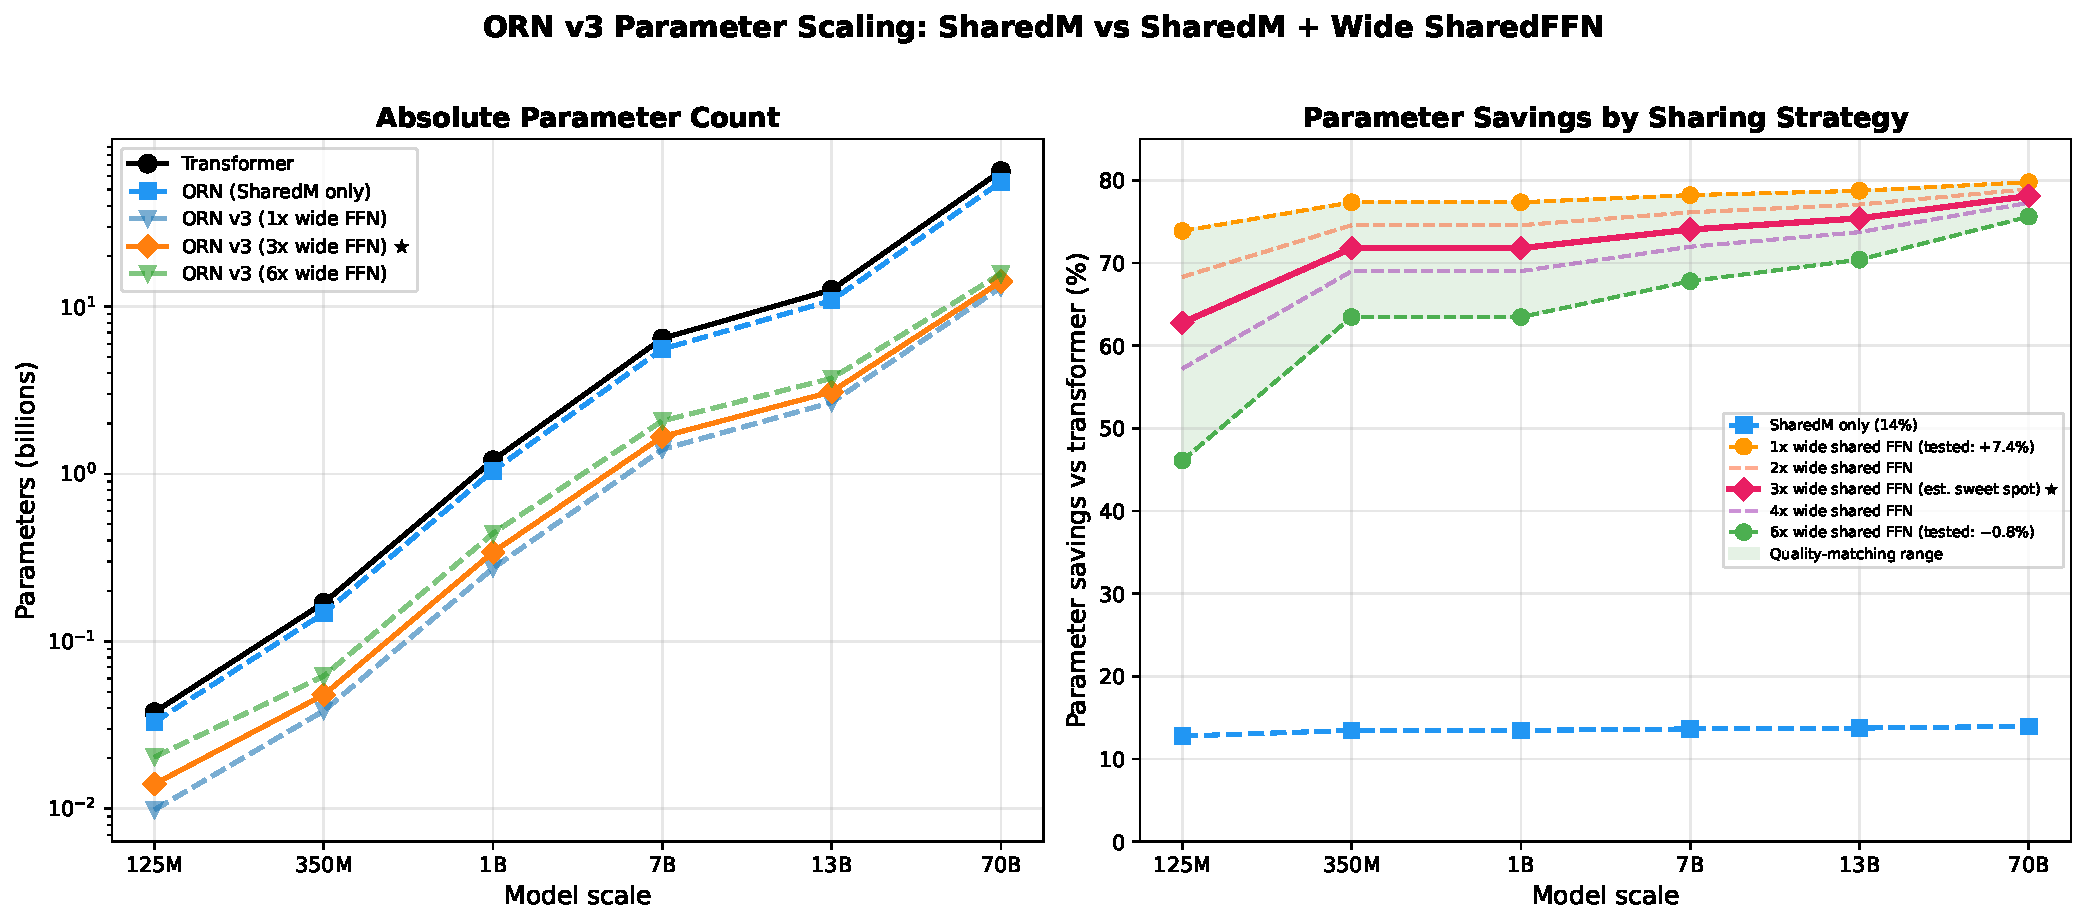
\includegraphics[width=\columnwidth]{orn_v3_scaling.pdf}
\caption{Parameter savings vs transformer across scales.
Blue dashed: SharedM only ($\sim$14\%).
Coloured: SharedM + wide shared FFN at various widths.
Green: quality-matching range ($1\times$: $+7.4\%$; $6\times$: $-0.8\%$).
For constrained deployment, $4\times$ (67\% budget, $+1.6\%$) is the practical sweet spot.}
\label{fig:scaling}
\end{figure}

\paragraph{V3 checkpoint comparison.}
At 3B tokens, the V3 model (61M params, $6\times$ wide shared FFN) produces better representations than V2 (108M, per-layer FFN, 4B tokens) on a curated 128-text evaluation corpus: full-embedding form classification 96.8\% vs 90.6\%, topic classification 82.0\% vs 78.2\%.
STS semantic similarity is matched (0.482 vs 0.489).
V3's $\M$ has higher effective rank (407 vs 332)---the wide shared FFN provides capacity alongside $\M$, so $\M$ uses more of the available dimensions rather than compressing aggressively.
Both models generate coherent multi-sentence English on diverse topics.
V3 achieves this at \textbf{56\% of V2's parameter count} with 75\% of the training tokens.

\paragraph{Benchmark profile.}
The benchmark profile (Table~\ref{tab:benchmarks}) evolved with training.
At 4B tokens, HellaSwag was the only benchmark where the \orn{} beat GPT-2 Small.
At 8B tokens (after WSD decay), the \orn{} wins on 5 of 8 tasks including ARC-Easy, ARC-Challenge, and BoolQ---tasks that reward factual knowledge.
The WSD decay phase was critical: ARC-Easy jumped from 30.5\% to 46.2\%, suggesting the decay phase allowed response heads to better exploit the coupling geometry for knowledge retrieval.
The remaining weaknesses---LAMBADA (exact next-word prediction, where brute-force data coverage helps) and WinoGrande (known to require $>$1B parameters)---are consistent with the \orn{}'s data efficiency advantage having limits.
The strongest relative performance is on structural reasoning tasks (HellaSwag, OpenBookQA), where shared coupling geometry provides an architectural advantage.

\paragraph{The correction gates as diagnostics.}
The perturbative correction gates (initialised off, learn to activate) provide a built-in diagnostic.
Gate magnitudes vary by modality (audio: 0.163, text: 0.106, images: 0.058), indicating where the mean-field coupling approximation is least sufficient.
This could inform where to invest additional per-layer capacity in production models.

\paragraph{SharedM forces syntax into the residual stream.}
A head-to-head comparison with GPT-2 Small reveals an unexpected property: the \orn{}'s residual stream carries \emph{much more} syntactic information than the transformer's.
Sentence pairs with the same syntactic structure but different content (``The cat chased the dog'' vs ``The bird ate the worm'') have position-wise cosine similarity 0.78 in the \orn{} and 0.996 in GPT-2.
Pairs with the same words but different syntax (``She saw him running'' vs ``Running, she saw him'') have cosine 0.44 in the \orn{} and 0.990 in GPT-2.

The syntactic separation (same-syntax cosine minus different-syntax cosine) is $0.35$ for the \orn{} versus $0.006$ for GPT-2---a $60\times$ difference.
GPT-2 produces nearly identical residual states regardless of syntactic structure because it can encode structural information in the \emph{per-layer weight differences} between its $L$ independent coupling matrices.
The \orn{} cannot: SharedM is identical at every layer, so the model \emph{must} encode syntax in the residual state.

This has a practical consequence: the residual stream becomes a syntactically structured manifold that is directly accessible to downstream computation.
In the transformer, syntactic information is distributed across $2L$ separate $W_Q, W_K$ matrices and must be extracted through layer-specific probing~\cite{hewitt2019probe}.
In the \orn{}, it lives in the residual stream, where a single linear operator can traverse it: a fitted $20 \times 20$ transition matrix reproduces the residual trajectory on unseen prompts with $>96.5\%$ cosine accuracy at all layers.

\paragraph{Toward composable coupling (\corn{}).}
Standard \orn{} layers form a pipeline: each layer expects specific intermediate representations from the previous one.
A composable variant---where $T(s) \circ T(t) \approx T(s+t)$ for the coupling operator---would enable variable-depth computation, native diffusion, and iterative refinement.
Our 4-modality results (Table~\ref{tab:multimodal}) show \corn{} beating the transformer on 3 of 4 modalities, and preliminary results show that the semigroup coupling parameter $t$ and the diffusion noise level $\sigma$ are numerically the same parameter.
This connection between coupling dynamics and generative modelling is explored in a companion paper.

\paragraph{Limitations.}
(1) The largest model is 108M parameters; we have not yet tested at 1B+, where the scaling advantage should be most visible.
(2) At 8B tokens the \orn{} beats both baselines on 5 of 8 benchmarks on average, but these baselines trained on 37--75$\times$ more data; comparisons against models with matched training compute are needed.
(3) V2 has trained on 8B tokens (of a planned 50B); val loss is still improving, and absolute quality comparisons against models trained on 300B+ tokens are premature.
(4) We have not tested the \orn{} as a drop-in replacement for $W_Q, W_K$ in existing pretrained transformers (post-hoc surgery fails; Table~\ref{tab:spectral} existence proof shows the geometry is there but cannot be extracted without end-to-end training).
(5) The spectral invariance finding has been measured on GPT-2 family and two other architectures; broader coverage (Llama, Mistral) would strengthen the claim.


% ======================================================================
\section{Conclusion}

Transformer attention coupling is spectrally redundant across layers.
The \orn{} exploits this by memoising the coupling rule as a single shared $\M = AB^\top$, achieving 24--48$\times$ coupling parameter compression with no quality loss at scale.
At 108M parameters, the \orn{} generates coherent English and beats GPT-2 Small on HellaSwag.
The coupling manifold is 5--8 dimensional---the relational grammar of language is a remarkably compact object.

The shared geometry transfers across datasets (1.4\% frozen-M gap), across domains (12--19\% transfer advantage), and across modalities (one $\M$ serving images, music, environmental sounds, and text).
These findings support the hypothesis that the coupling rule is a universal structural property of the data, not a per-layer learned function.

All code, checkpoints, and experiment scripts are publicly available.


% ======================================================================
\small
\bibliographystyle{plainnat}
\begin{thebibliography}{99}

\bibitem{vaswani2017attention}
A.~Vaswani et al.
\newblock Attention Is All You Need.
\newblock \emph{NeurIPS}, 2017.

\bibitem{lan2020albert}
Z.~Lan et al.
\newblock ALBERT: A Lite BERT for Self-supervised Learning of Language Representations.
\newblock \emph{ICLR}, 2020.

\bibitem{xiao2019sharing}
Y.~Xiao et al.
\newblock Sharing Attention Weights for Fast Transformer.
\newblock \emph{IJCAI}, 2019.

\bibitem{takase2021sharing}
S.~Takase and S.~Kiyono.
\newblock Lessons on Parameter Sharing across Layers in Transformers.
\newblock \emph{arXiv:2104.06022}, 2021.

\bibitem{masa2025}
Share Your Attention: Transformer Weight Sharing via Matrix-based Dictionary Learning.
\newblock \emph{arXiv:2508.04581}, 2025.

\bibitem{reid2021reuse}
Leveraging Redundancy in Attention with Reuse Transformers.
\newblock \emph{arXiv:2110.06821}, 2021.

\bibitem{dehghani2018universal}
M.~Dehghani et al.
\newblock Universal Transformers.
\newblock \emph{ICLR}, 2019.

\bibitem{gu2023mamba}
A.~Gu and T.~Dao.
\newblock Mamba: Linear-Time Sequence Modeling with Selective State Spaces.
\newblock \emph{arXiv:2312.00752}, 2023.

\bibitem{lieber2024jamba}
O.~Lieber et al.
\newblock Jamba: A Hybrid Transformer-Mamba Language Model.
\newblock \emph{arXiv:2403.19887}, 2024.

\bibitem{katharopoulos2020transformers}
A.~Katharopoulos et al.
\newblock Transformers are RNNs: Fast Autoregressive Transformers with Linear Attention.
\newblock \emph{ICML}, 2020.

\bibitem{dao2022flashattention}
T.~Dao et al.
\newblock FlashAttention: Fast and Memory-Efficient Exact Attention with IO-Awareness.
\newblock \emph{NeurIPS}, 2022.

\bibitem{he2016deep}
K.~He et al.
\newblock Deep Residual Learning for Image Recognition.
\newblock \emph{CVPR}, 2016.

\bibitem{qk2024eigenspectrum}
Self-attention Networks Localize When QK-eigenspectrum Concentrates.
\newblock \emph{arXiv:2402.02098}, 2024.

\bibitem{spectral2024rankcollapse}
Mind the Gap: A Spectral Analysis of Rank Collapse and Signal Propagation in Attention Layers.
\newblock \emph{arXiv:2410.07799}, 2024.

\bibitem{brunton2022data}
S.~Brunton and J.~Kutz.
\newblock \emph{Data-Driven Science and Engineering: Machine Learning, Dynamical Systems, and Control}.
\newblock Cambridge University Press, 2nd edition, 2022.

\bibitem{kornblith2019cka}
S.~Kornblith et al.
\newblock Similarity of Neural Network Representations Revisited.
\newblock \emph{ICML}, 2019.

\bibitem{ainslie2023gqa}
J.~Ainslie et al.
\newblock GQA: Training Generalized Multi-Query Transformer Models from Multi-Head Checkpoints.
\newblock \emph{EMNLP}, 2023.

\bibitem{su2024rope}
J.~Su et al.
\newblock RoFormer: Enhanced Transformer with Rotary Position Embedding.
\newblock \emph{Neurocomputing}, 2024.

\bibitem{mcclelland1995complementary}
J.~L.~McClelland et al.
\newblock Why There Are Complementary Learning Systems in the Hippocampus and Neocortex.
\newblock \emph{Psychological Review}, 102(3):419--457, 1995.

\bibitem{onewideffn2023}
A.~Pires, A.~Lopes et al.
\newblock One Wide Feedforward is All You Need.
\newblock \emph{WMT at EMNLP}, 2023.

\end{thebibliography}

\end{document}
